\documentclass{book}
\usepackage{explorations}
\usepackage[subpreambles=false]{standalone}
\usepackage{import}
\usepackage[subfigure]{tocloft}


\tikzset{
  piechart/.pic={
    \draw (0,0) circle (2cm);
    \draw[very thick, fill=cba] (0,0) -- (-90:2) arc(-90:54:2) -- cycle;
    \node at (-18:1)  {Exams};
    \draw[very thick, fill=cbb] (0,0) -- (54:2) arc(54:108:2) -- cycle;
    \node at (81:1.5) {Project};
    \draw[very thick, fill=cbc] (0,0) -- (108:2) arc(108:162:2) -- cycle;
    \node at (135:1.4) {\small In class};
    \draw[very thick, fill=cbd] (0,0) -- (162:2) arc(162:198:2) -- cycle;
    \node[anchor=west] at (180:2) {HW};
    \draw[very thick, fill=cbe] (0,0) -- (198:2) arc (198:270:2) -- cycle;
    \node at (234:1.2) {Final};
  }
}
  
\title{What}

%\let\cleardoublepage\clearpage
\course{Explorations 1}

\begin{document}
\frontmatter
\pagestyle{plain}



\begin{titlepage}
  \

  \vfill
  
  \begin{center}
    \Large\textsf{\textsc{San Diego City College\\ Math 59 --- Explorations I\\ Modules 0--7}}
  \end{center}

  \vfill
 
  \begin{center}
    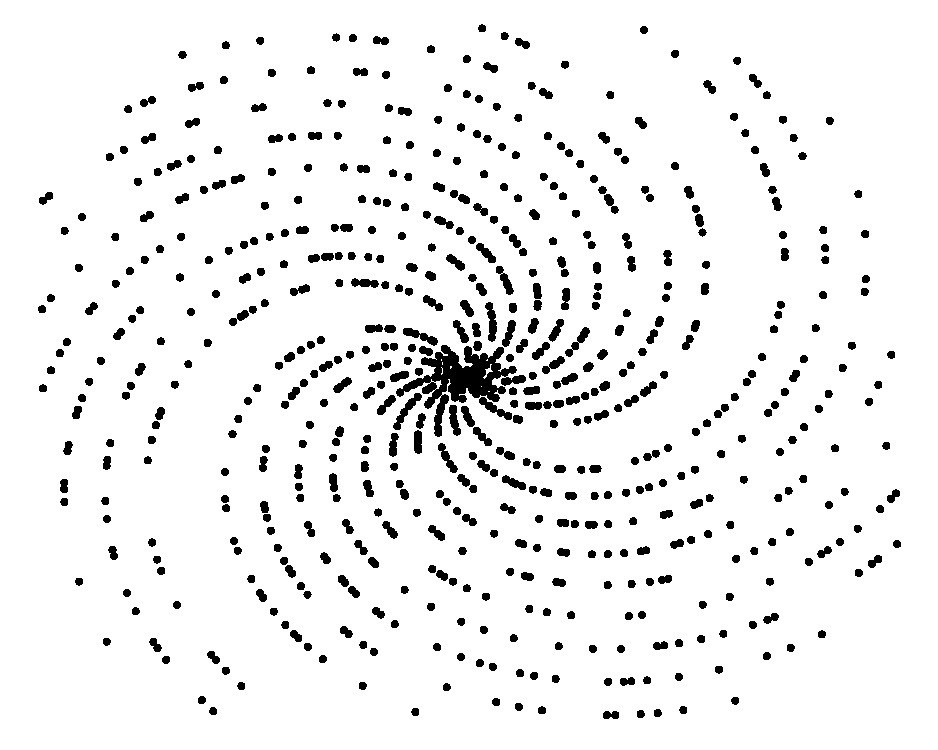
\includegraphics{primespiral.pdf}
  \end{center}

  \vfill
  
\end{titlepage}

% \addtocounter{page}{-1}
\setcounter{tocdepth}{0}
\setcounter{secnumdepth}{-2}
% \renewcommand{\cfttoctitlefont}{\Huge\sffamily\bfseries}
% \renewcommand{\cftpartfont}{\LARGE\sffamily}
% \renewcommand{\cftpartpagefont}{\LARGE\sffamily}
\tableofcontents

\mainmatter
\pagestyle{fancy}

\part{Module 0}

\module{Module 0}

\lesson{0.0.0.1 --- Introduction}
\graphicspath{{module0/0.0.0.1-introduction/}}
\lesson{What}
\import{module0/0.0.0.1-introduction/}{0.0.0.1-introduction.tex}

\mynewpage

\thispagestyle{plain}
\begin{center}
  \Large People Bingo
\end{center}
\begin{itemize}
\item Find someone who matches each characteristic and ask them to sign in the box.
\item You can't have the same person sign more than one box on your paper.
\end{itemize}

\begin{center}
  \begin{tikzpicture}[x=1in,y=1in,scale=0.9]
    \draw[step=2in,black,thick] (0,0) grid (8,8);
    \node[anchor=north, align=center, text width = 1.75in] at (1,8) {Is Married};
    \node[anchor=north, align=center, text width = 1.75in] at (3,8) {Has Children};
    \node[anchor=north, align=center, text width = 1.75in] at (5,8) {Lives more than 10 miles from campus};
    \node[anchor=north, align=center, text width = 1.75in] at (7,8) {Speaks a language other than English};
    \node[anchor=north, align=center, text width = 1.75in] at (1,6) {Lived outside of the US};
    \node[anchor=north, align=center, text width = 1.75in] at (3,6) {Plays a musical instrument};
    \node[anchor=north, align=center, text width = 1.75in] at (5,6) {Wears glasses or contacts};
    \node[anchor=north, align=center, text width = 1.75in] at (7,6) {Is under 21 years of age};
    \node[anchor=north, align=center, text width = 1.75in] at (1,4) {Is left-handed};
    \node[anchor=north, align=center, text width = 1.75in] at (3,4) {Is vegetarian or vegan};
    \node[anchor=north, align=center, text width = 1.75in] at (5,4) {Works full- or part-time};
    \node[anchor=north, align=center, text width = 1.75in] at (7,4) {Plays video games};
    \node[anchor=north, align=center, text width = 1.75in] at (1,2) {Exercises Regularly};
    \node[anchor=north, align=center, text width = 1.75in] at (3,2) {Does Not Have a Facebook Account};
    \node[anchor=north, align=center, text width = 1.75in] at (5,2) {Has a January Birthday};
    \node[anchor=north, align=center, text width = 1.75in] at (7,2) {Other:\\ \ \\ \underline{\hspace{1.5in}}};
  \end{tikzpicture}
\end{center}

\newpage
\thispagestyle{plain}
\ 

\part{Module 1}

\pagestyle{fancy}

\module{Module 1} 

\lesson{1.0.0.1 --- Introduction}
% \addcontentsline{toc}{chapter}{1.0.0.1 --- Introduction}
\graphicspath{{module1/1.0.0.1-introduction/}}
\import{module1/1.0.0.1-introduction/}{1.0.0.1-introduction.tex}
\mynewpage

\lesson{1.0.0.1 --- Pie Charts}
% \addcontentsline{toc}{chapter}{1.0.0.2 --- Pie Charts}
\graphicspath{{module1/1.0.0.2-pie-charts/}}
\import{module1/1.0.0.2-pie-charts/}{1.0.0.2-pie-charts.tex}
\mynewpage

\lesson{1.1.2.1 --- Real Numbers}
\graphicspath{{module1/1.1.2.1-real-numbers/}}
\import{module1/1.1.2.1-real-numbers/}{1.1.2.1-real-numbers.tex}
\mynewpage

\lesson{1.2.0.2 --- Money Stacks}
\graphicspath{{module1/1.2.0.2-money-stacks/}}
\import{module1/1.2.0.2-money-stacks/}{1.2.0.2-money-stacks.tex}

\mynewpage

\lesson{1.2.0.4 --- Powers of 2, \nicefrac{1}{2}, and 10}
\graphicspath{{module1/1.2.0.4-powers-of-two/}}
\import{module1/1.2.0.4-powers-of-two/}{1.2.0.4-powers-of-two.tex}


\end{document}
%%% Local Variables:
%%% mode: latex
%%% TeX-master: t
%%% TeX-engine: default
%%% End:
